\documentclass[handout,compress]{beamer}

\usetheme[block=fill]{metropolis}

\usepackage{graphicx} % Allows including images
\usepackage{amsmath,amsfonts,amsthm,amssymb}
\usepackage{color}
\usepackage{xcolor,cancel}
%\setitemize{label=\usebeamerfont*{itemize item}%
%	\usebeamercolor[fg]{itemize item}
%	\usebeamertemplate{itemize item}}
\definecolor{mDarkBrown}{HTML}{604c38}
\definecolor{mDarkTeal}{HTML}{23373b}
\definecolor{mLightBrown}{HTML}{EB811B}
\definecolor{mMediumBrown}{HTML}{C87A2F}
\definecolor{mygreen}{HTML}{98C2B9}
\definecolor{myyellow}{HTML}{DFD79C}
\definecolor{myblue}{HTML}{8CA7CC}
\definecolor{kern}{HTML}{8CC2B7}

\usepackage{float}
\usepackage{framed}
\usepackage{epsfig}
\usepackage{graphicx}
\usepackage{subcaption}
\usepackage{ulem}
\usepackage{hhline}
\usepackage{multirow}
\usepackage{comment}   
\usepackage{bbm}
\usepackage{tikz}   
\usepackage{ulem}
\def\Put(#1,#2)#3{\leavevmode\makebox(0,0){\put(#1,#2){#3}}}
\newcommand*\mystrut[1]{\vrule width0pt height0pt depth#1\relax}
\newcommand{\eqdef}{\mathbin{\stackrel{\rm def}{=}}}


\newcommand{\bs}[1]{\boldsymbol{#1}}
\newcommand{\bv}[1]{\mathbf{#1}}
\newcommand{\R}{\mathbb{R}}
\newcommand{\E}{\mathbb{E}}

\DeclareMathOperator*{\argmin}{arg\,min}
\DeclareMathOperator*{\argmax}{arg\,max}
\DeclareMathOperator{\nnz}{nnz}
\DeclareMathOperator{\Var}{Var}
\DeclareMathOperator{\sinc}{sinc}
\DeclareMathOperator{\mv}{mv}
\DeclareMathOperator{\sgn}{sgn}
\DeclareMathOperator{\step}{step}
\DeclareMathOperator{\gap}{gap}
\DeclareMathOperator{\poly}{poly}
\DeclareMathOperator{\tr}{tr}
\DeclareMathOperator{\orth}{orth}
\newcommand{\norm}[1]{\|#1\|}
\captionsetup[subfigure]{labelformat=empty}
\captionsetup[figure]{labelformat=empty}
\DeclareMathOperator*{\lmin}{\lambda_{min}}
\DeclareMathOperator*{\lmax}{\lambda_{max}}

\newcommand{\specialcell}[2][c]{%
  \begin{tabular}[#1]{@{}c@{}}#2\end{tabular}}
\newcommand{\specialcellleft}[2][c]{%
\begin{tabular}[#1]{@{}l@{}}#2\end{tabular}
}

\usepackage{tabstackengine}
\stackMath

\newtheorem{claim}[theorem]{Claim}


%----------------------------------------------------------------------------------------
%	TITLE PAGE
%----------------------------------------------------------------------------------------

\title{CS-UY 4563: Lecture 11 \\ Finish-Up Gradient Descent, Midterm Review}
\author{NYU Tandon School of Engineering, Prof. Christopher Musco}
\date{}

\begin{document}

\begin{frame}
	\titlepage 
\end{frame}

\metroset{titleformat=smallcaps}

\begin{frame}
	\frametitle{gradient descent}
	\begin{itemize}
		\item We want to choose $\vec{\beta}$ to minimize a loss function $L(\vec{\beta})$.
		\item Often we can compute $\nabla L(\vec{\beta})$ for any $\vec{\beta}$, but can't explicitly find a $\vec{\beta}^*$ for which $\nabla L(\vec{\beta}) = \vec{0}$. 
		\item Instead, we \emph{iteratively search} a near optimal $\vec{\beta}$.
	\end{itemize}
\end{frame}

\begin{frame}
	\frametitle{gradient descent}
	\textbf{Gradient descent algorithm for minimizing $L(\vec{\beta})$:}
	\begin{itemize}
		\item Choose arbitrary starting point $\vec{\beta}^{(0)}$.
		\item For $i = 1,\ldots, T$:
		\begin{itemize}
			\item $\vec{\beta}^{(i+1)} = \vec{\beta}^{(i)} - \eta \nabla L(\vec{\beta}^{(i)})$
		\end{itemize}
		\item Return $\vec{\beta}^{(t)}$.
	\end{itemize}
	Or stop after $L(\beta^{(i)})$ stops decreasing.

	$\eta$ is a \emph{step-size} parameter. Also called the \emph{learning rate}. Needs to be chosen sufficiently small for gradient descent to converge, but too small will slow down the algorithm. 
\end{frame}

\begin{frame}
	\frametitle{learning rate}
	Precision in choosing the learning rate $\eta$ is not super important, but we do need to get it to the right order of magnitude. 
	\begin{center}
		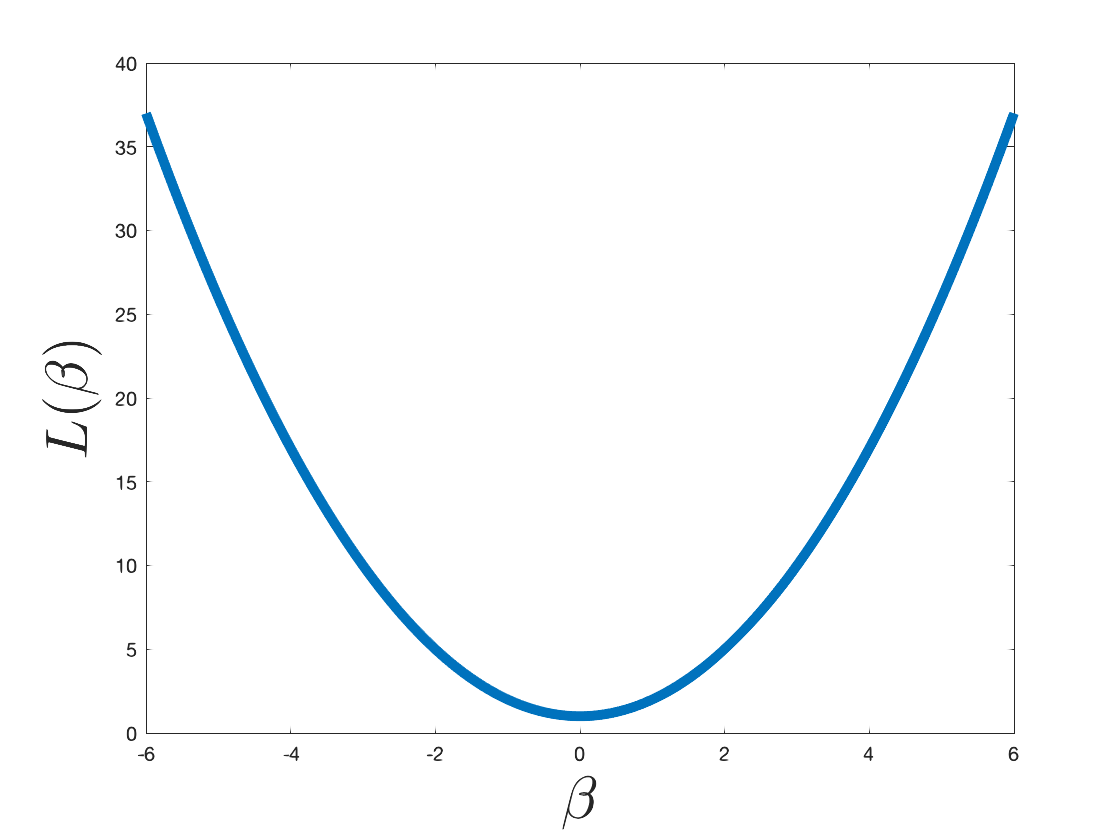
\includegraphics[width=.7\textwidth]{simple1d.png}
	\end{center}
\end{frame}

\begin{frame}
	\frametitle{learning rate}
	``Overshooting'' can be a problem if you choose the step-size too high. 
	\begin{center}
		\includegraphics[width=.3\textwidth]{too_slow.png} 	\includegraphics[width=.3\textwidth]{just_right.png} 	\includegraphics[width=.3\textwidth]{too_fast.png}
	\end{center}
	Often a good idea to plot the \emph{entire optimization} curve for diagnosing what's going on.
	
	We will have a mini-lab on gradient descent optimization after the midterm we're you'll get practice doing this.
\end{frame}

\begin{frame}
	\frametitle{exponential grid search}
	Just as in regularization, search over a grid of possible parameters:
	\begin{align*}
	\eta = [2^{-5}, 2^{-4}, 2^{-3}, \ldots, 2^9,2^{10}].
	\end{align*}
	Or tune by hand based on the optimization curve.
\end{frame}

\begin{frame}
	\frametitle{backtracking  line search/armijo rule}
	\textbf{Recall}: If we set $\vec{\beta^{(i+1)}}\leftarrow \vec{\beta^{(i)}} - \eta \nabla L(\vec{\beta^{(i)}})$ then:
	\begin{align*}
		L(\vec{\beta^{(i+1)}}) &\approx L(\vec{\beta^{(i)}}) - \eta \langle \nabla L(\vec{\beta^{(i)}}), \nabla L(\vec{\beta^{(i)}})\rangle\\
		 &= L(\vec{\beta^{(i)}}) - \eta  \|\nabla L(\vec{\beta^{(i)}})\|_2^2.
	\end{align*}
	\begin{center}
		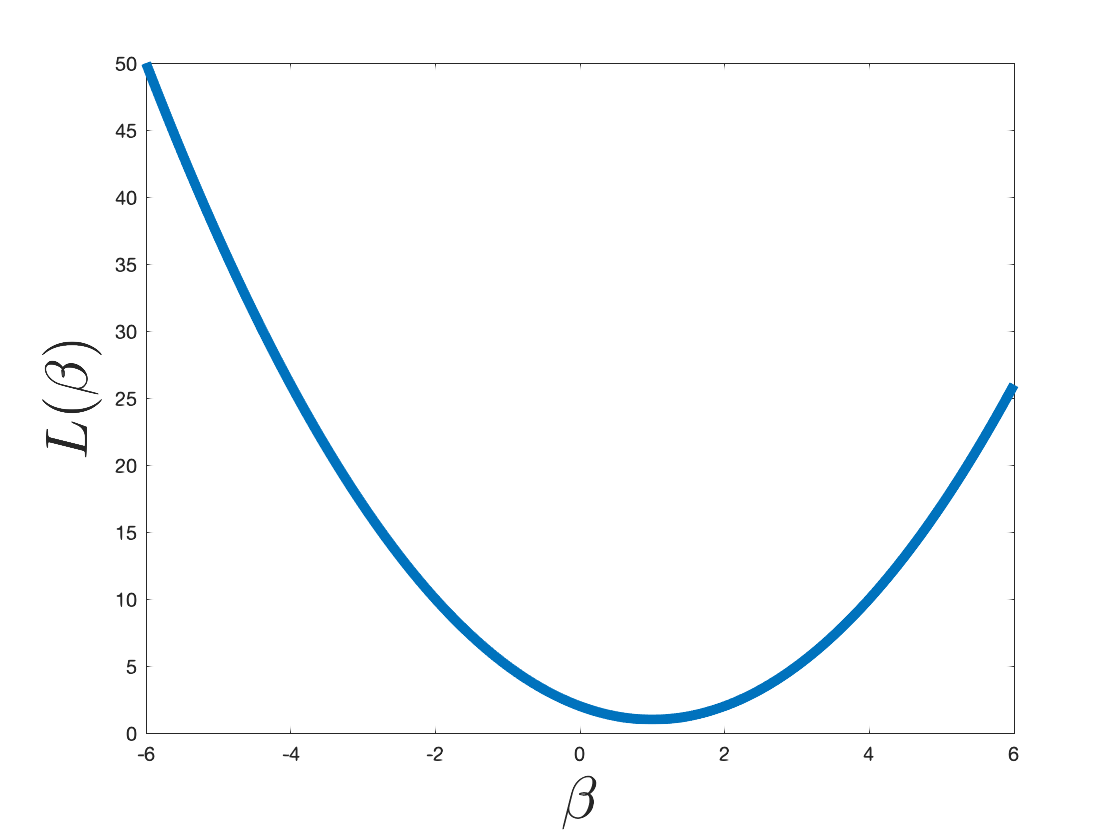
\includegraphics[width=.4\textwidth]{1d_example.png}
		
		Approximation holds true for small $\eta$. When it does not, we might be overshooting.
	\end{center}
\end{frame}

\begin{frame}
	\frametitle{backtracking  line search/armijo rule}
	\small
	\textbf{Gradient descent with backtracking line search:}
	\begin{itemize}
		\item Choose arbitrary starting point $\vec{\beta}$.
		\item Choose starting step size $\eta$. 
		\item Choose $\tau, c < 1$ (typically both $c = 1/2$ and $\tau = 1/2$)
		\item For $i = 1,\ldots, T$:
		\begin{itemize}
			\item $\vec{\beta}^{(new)} = \vec{\beta} - \eta \nabla L(\vec{\beta})$
			\item If $L(\vec{\beta}^{(new)}) \leq L(\vec{\beta}) - c\eta  \|\nabla L(\vec{\beta})\|_2^2$
				\begin{itemize}
					\item $\vec{\beta} \leftarrow \vec{\beta}^{(new)}$
					\item $\eta \leftarrow \tau^{-1}\eta$
				\end{itemize}
			\item Else
				\begin{itemize}
					\item $\eta \leftarrow \tau\eta$
				\end{itemize}
		\end{itemize}
	\end{itemize}
\textbf{\alert{Always decreases objective value, works very well in practice.}}
\end{frame}

\begin{frame}[t]
	\frametitle{convergence of gradient descent}
	\begin{center}
		\textbf{In general GD only converges to a \alert{local minimum}.}
		
		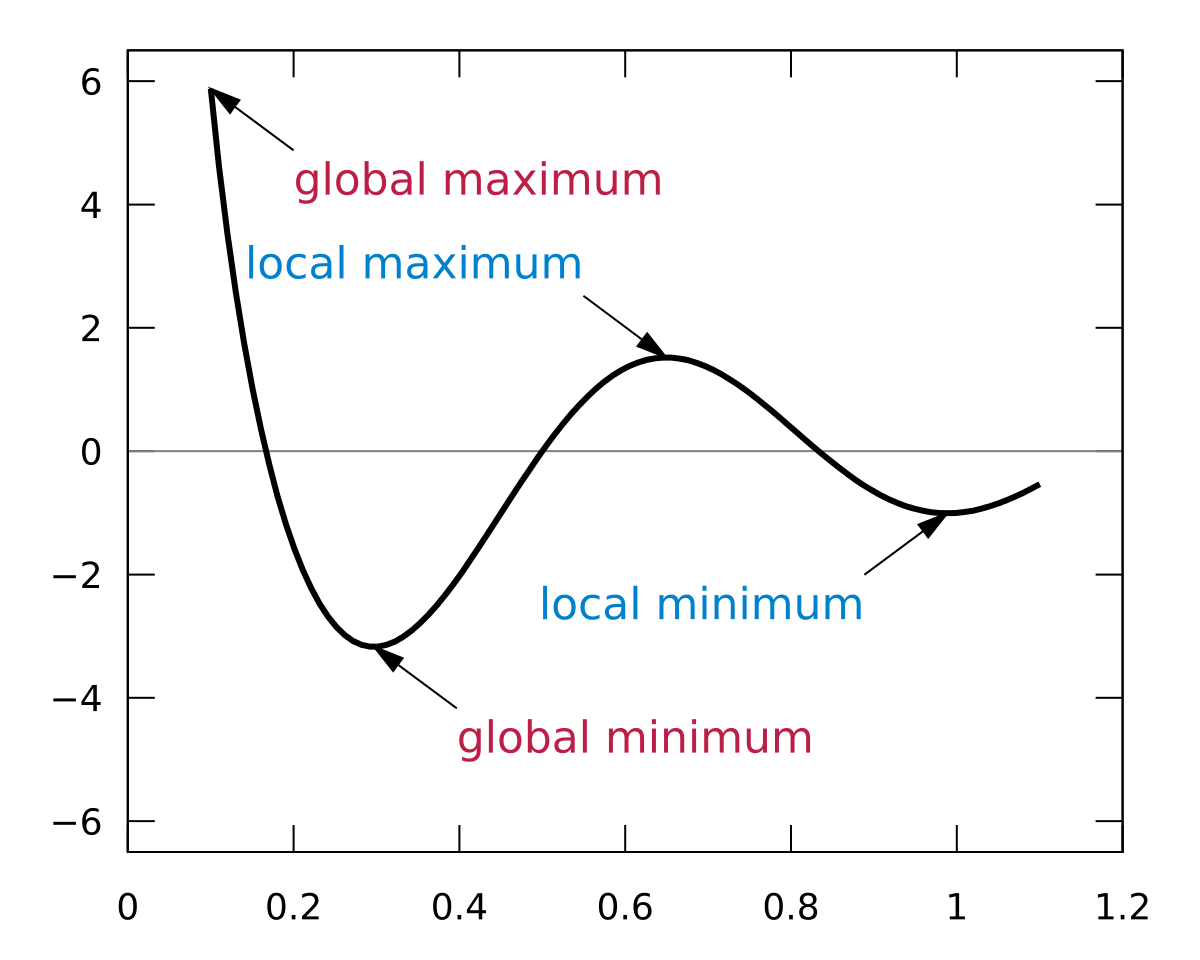
\includegraphics[width=.7\textwidth]{local_min.png}
	\end{center}
\end{frame}

\begin{frame}[t]
	\frametitle{convex function}
		\begin{definition}[Convex]
		A function $L$ is convex iff for any $\vec{\beta_1}, \vec{\beta_2},\lambda \in [0,1]$:
		\begin{align*}
		(1-\lambda)\cdot L(\vec{\beta_1}) + \lambda \cdot L(\vec{\beta_2}) \geq L\left((1-\lambda)\cdot\vec{\beta_1}+ \lambda \cdot\vec{\beta_2}\right)
		\end{align*}
		\vspace{-1em}
	\end{definition}
\vspace{-2em}
\begin{center}
	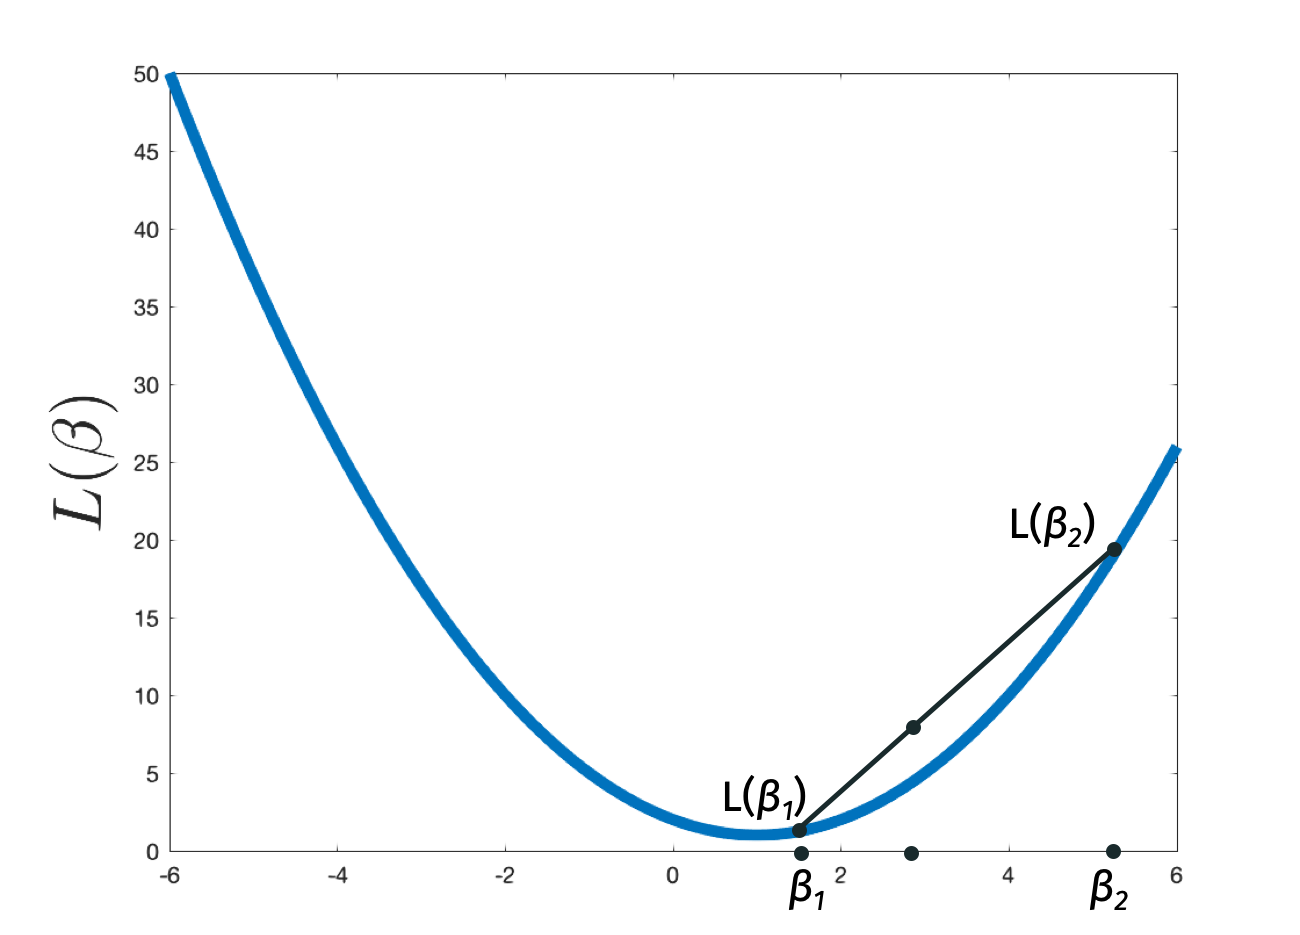
\includegraphics[width=.75\textwidth]{convex.png}
\end{center}
\end{frame}

\begin{frame}
		\frametitle{convex function}
	\textbf{In words:} A function is convex if a line between any two points on the function lies above the function. Captures the notion that a function looks like a bowl.
	
	\begin{center}
				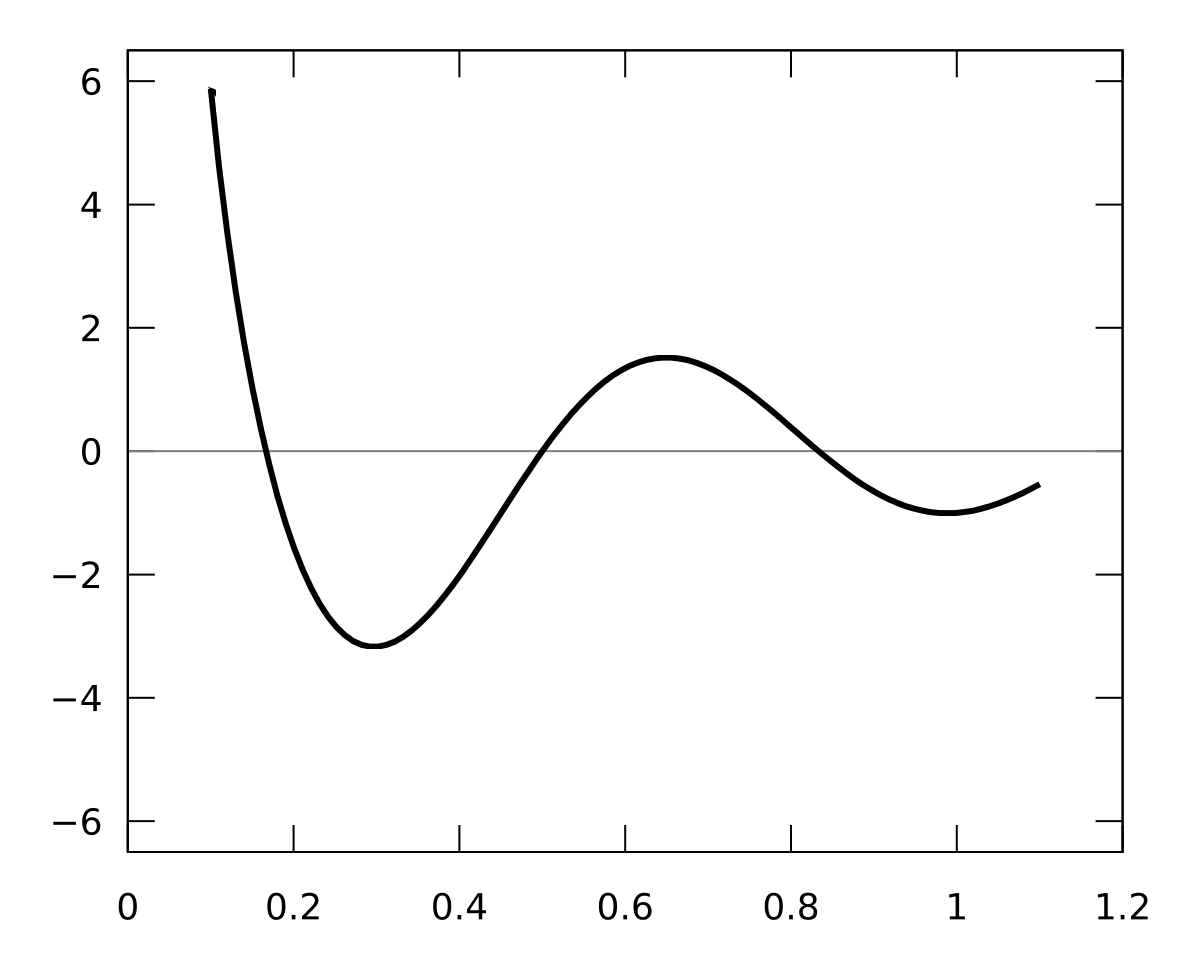
\includegraphics[width=.7\textwidth]{local_min_blank.png}
				
		This function is \textbf{not} convex.
	\end{center} 
	
\end{frame}

\begin{frame}[t]
	\frametitle{convex function}
		\begin{claim}[Convex Function Minimizers.]
		Every \emph{local} minimum of a convex function is also a \emph{global minimum}.
	\end{claim}
	\begin{center}
	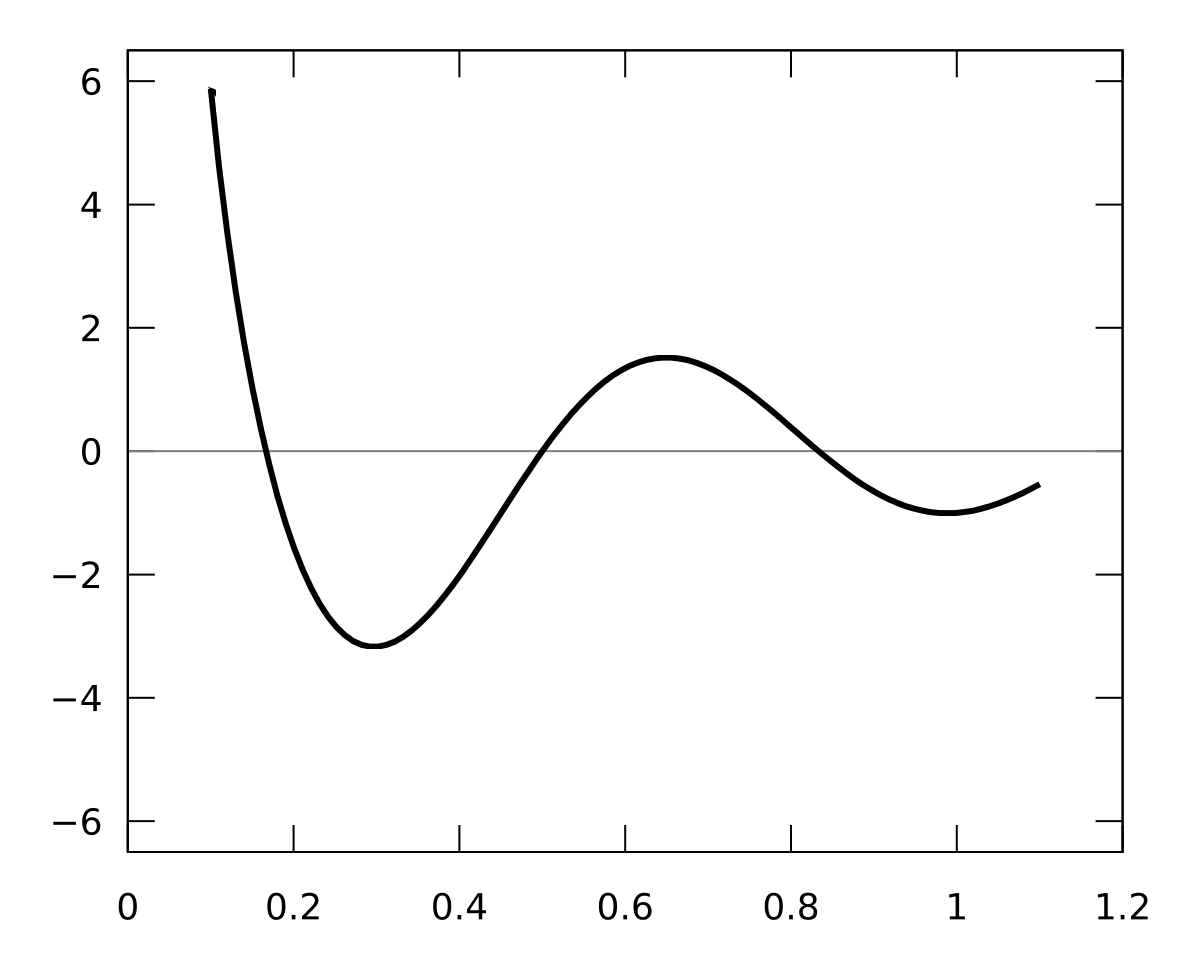
\includegraphics[width=.7\textwidth]{local_min_blank.png}
	\end{center} 
\end{frame}

\begin{frame}[t]
	\frametitle{convergence of gradient descent}
	\begin{claim}[GD Convergence for Convex Functions.]
		For sufficiently small step-size $\eta$, Gradient Descent converges to an approximate global minimum of any convex function $L$.
	\end{claim}

	\textbf{What functions are convex?}
	\begin{itemize}
		\item Least squares loss for linear regression.
		\item $\ell_1$ loss for linear regression.
		\item Either of these with and $\ell_1$ or $\ell_2$ regularization penalty. 
		\item Logistic regression! Logistic regression with regularization.
		\item Many other models in machine leaning!
	\end{itemize}
\begin{center}
	\textbf{This is not a coincidence:} often it makes sense to reformulate your problem so that the loss function is convex, simply so you can minimize it with GD. 
\end{center}
\end{frame}

\begin{frame}[standout]
	midterm review
\end{frame}

\begin{frame}
	\frametitle{data transformations}
	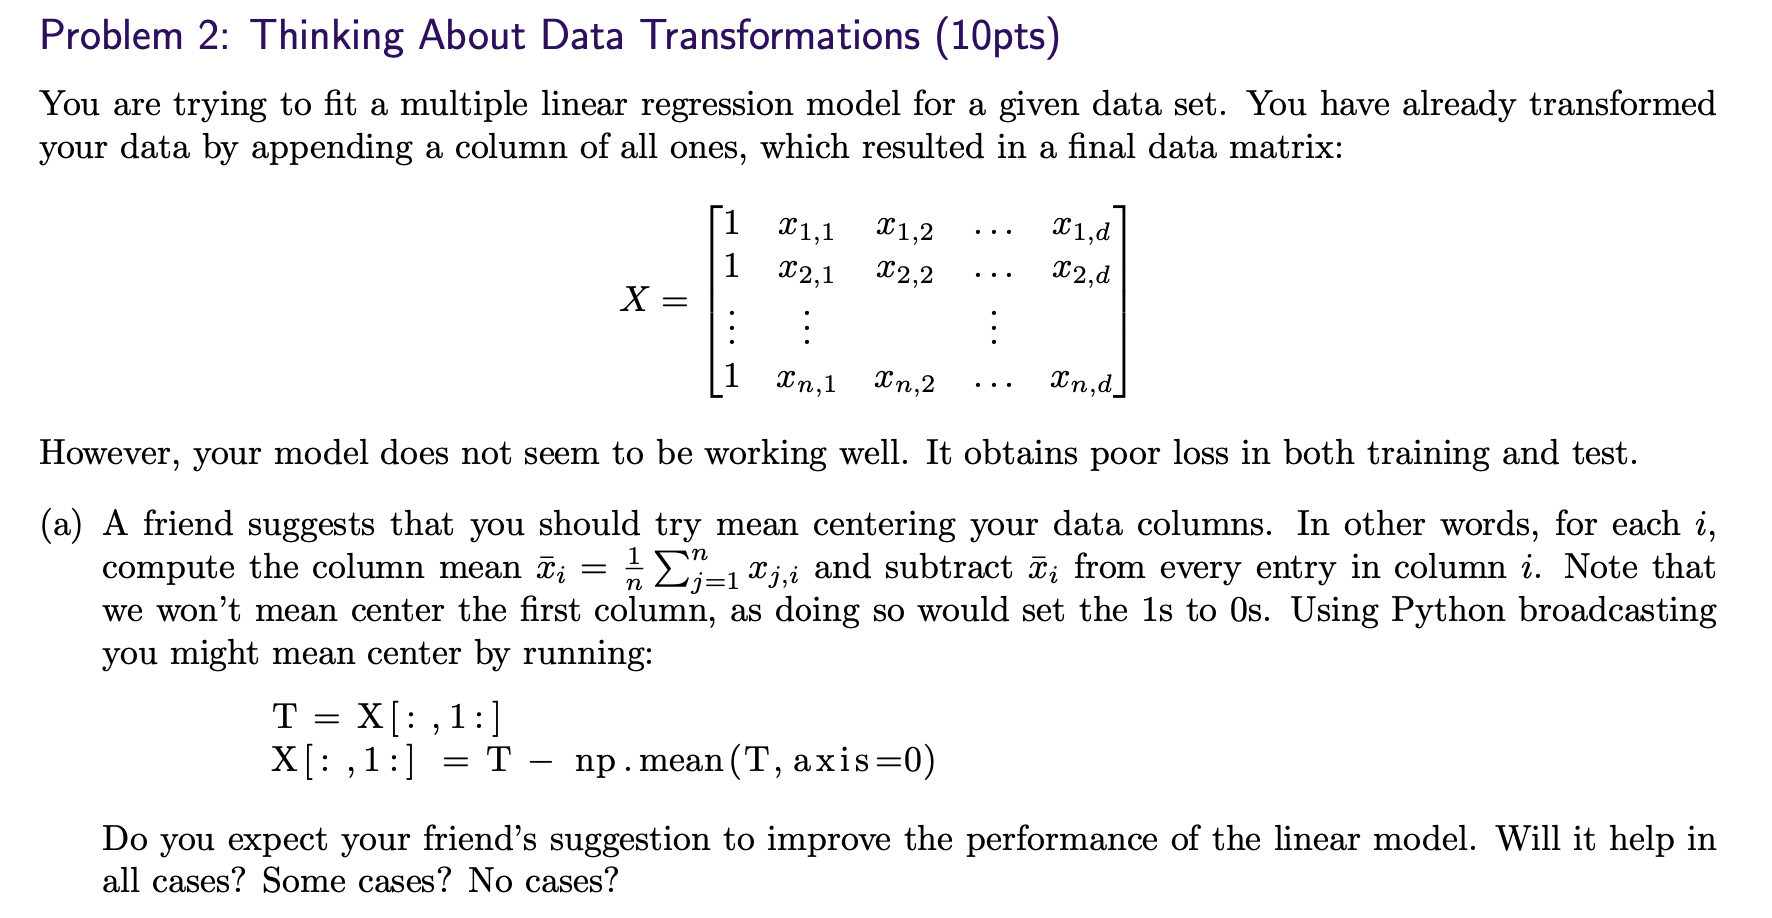
\includegraphics[width=\textwidth]{data_transformations.png}
	
\end{frame}

\begin{frame}
	\frametitle{mean centering has no effect on linear regression}
\end{frame}

\begin{frame}
	\frametitle{mean centering has no effect on linear regression}
\end{frame}

\begin{frame}
	\frametitle{column scaling has no effect on linear regression}
\end{frame}

\begin{frame}
	\frametitle{column scaling has no effect on linear regression}
\end{frame}

\begin{frame}[t]
	\frametitle{data transformations for temporal data}
	\textbf{Electrocorticography ECoG lab:}
	\begin{itemize}
		\item Implant grid of electrodes on surface of monkey's brain to measure electrical activity in different regions. 
	\end{itemize} 
	\begin{center}
		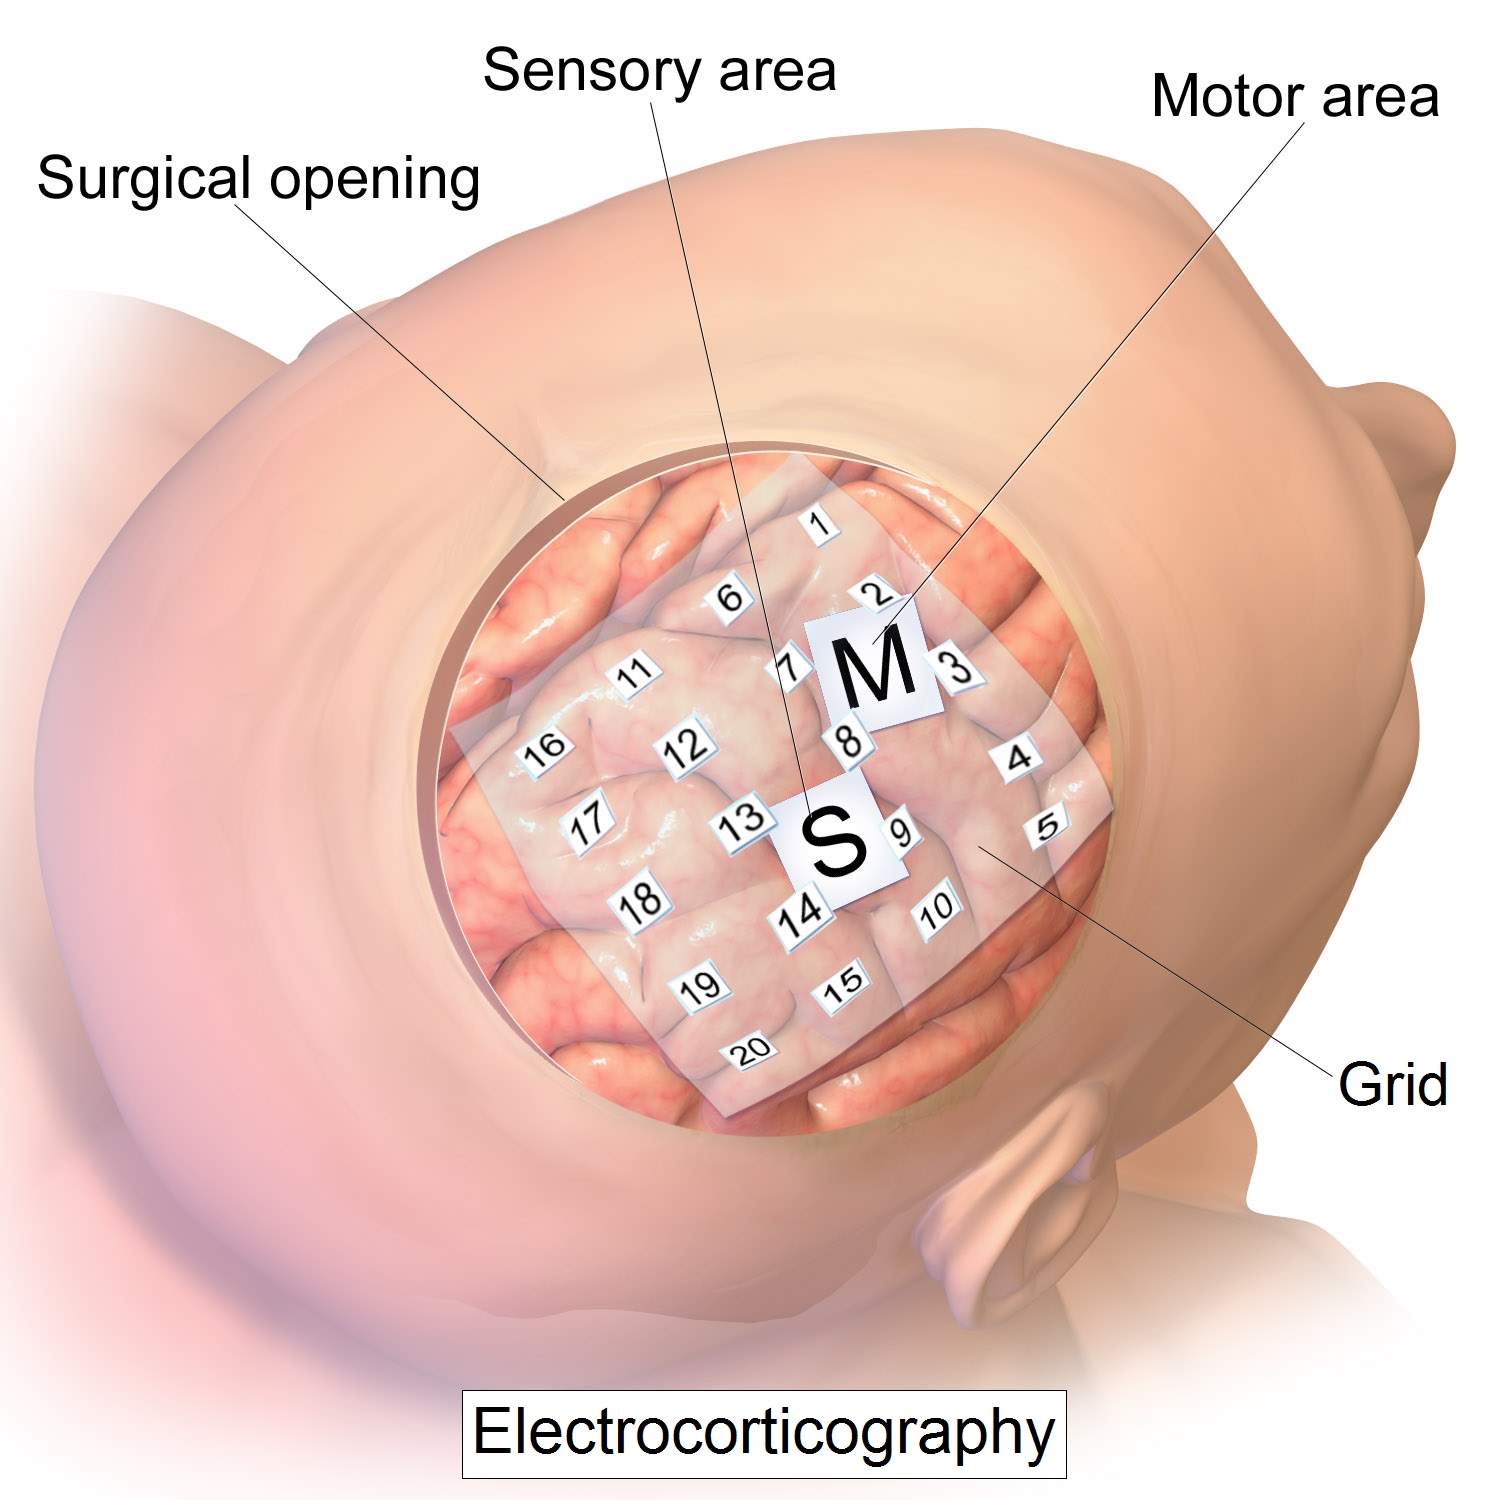
\includegraphics[width=.3\textwidth]{eocg.png}
	\end{center}
	\begin{itemize}
		\item Predict hand motion based on 53 ECoG measurements.
		\item \textbf{Model order:} predict movement at time $t$ using brain signals at time $t,t-1, \ldots, t-q$ for varying values of $q$. 
	\end{itemize} 
\end{frame}

\begin{frame}[t]
	\frametitle{data transformations for temporal data}
\end{frame}

\begin{frame}[t]
	\frametitle{data transformations for temporal data}
\end{frame}

\end{document} 






